%%!TEX TS-program = latex
\documentclass[12pt,letterpaper]{article}
\usepackage{epsfig}                 
\usepackage[authoryear]{natbib}
\usepackage{graphicx}
\usepackage{amsmath}
\usepackage{psfrag}
\usepackage{mathabx}
\renewcommand{\baselinestretch}{1.6}
\large
\pagenumbering{arabic}
\usepackage[usenames,dvipsnames]{color}
\usepackage{fullpage}
\bibliographystyle{genetics}
\usepackage{multirow}
\newcommand{\ye}{\hat{y}}
\newcommand{\xe}{\hat{x}}
\usepackage{color}
\usepackage[normalem]{ulem}  
	\newcommand{\gc}[1]{{ \color{red} #1}}
	\newcommand{\yb}[1]{{ \color{blue} #1}}




%Why do animals allow male control of female meiosis?

%Why does female meiosis allow the opportunity for exploitation by selfish sperm?


%sperm and egg genomes both favour the peaceful resolution of female meiotic drive
%strange bed fellows

\title{Why does female meiosis allow the opportunity for exploitation
  by selfish sperm? BETTER TITLE?}
\author{Yaniv Brandvain \\ email: ybrandvain@gmail.com  \and Graham Coop \\ email: gmcoop@ucdavis.edu }

\usepackage{fancyhdr}
\pagestyle{fancy}
\lhead{}
\rhead{}
\renewcommand{\headrulewidth}{0.0pt}
\rfoot{}
\cfoot{\thepage}
\date{}
\bibliographystyle{plain}
\begin{document}
\maketitle
\begin{center}
Center for Population Biology \& Department of Evolution and Ecology \\ University of California - Davis \\ Davis, CA, 95616
\end{center}

%FIgures 
{\bf Abstract:}
\newpage

\section*{Introduction}

%Since all alleles within an individual rely on individual survival and reproduction for evolutionary success, most of life in a diploid eukaryotic genome is harmonious.
%However, this harmony is incomplete, as in numerous cases an allele can benefit (in the short or long term) from taking advantage of its host.
Despite the apparent unity of the organism, occasionally alleles can
gain an evolutionary advantage at a cost to  individual fitness
\citep{Burt2006}, often by exploiting meiosis and gametogensis.
%A clear opportunity for this conflict arises during gametogenesis where alternative alleles are in direct competition for representation in the next generation.
Because only one of the four products of female meiosis is transmitted to the egg, female meiosis \yb{is particularly vulnerable to such exploitation}  \citep{Sandler1957,Pardo-ManuelDeVillena2001a}. 
%Female meiosis is particularly unfair, only one of the four products of meiosis becomes an egg, while the other threes are disgarded into polar bodies. 
An allele that biases female meiosis in its favor (i.e. a meiotic driver), may increase in frequency even if this driver entails a pleiotropic fitness cost \citep{Prout1973}, generating a genetic conflict between the success of the driver and organismal fitness.
%Alleles that can segregate into the egg more than half the time in heterozygotes, by exploiting asymmetries, 
%can potentially increase in frequency in the population (i.e. experiencing true meiotic drive).
%If such alleles have fitness consequences they are a source of genetic conflict, 
%and can become balanced in the population if their host in homozygotes 
%out weighs their ability to spread to spread through heterozygotes. 
Meiotic drivers observed in nature (in both plants
\citep{Buckler1999,Fishman2005,Fishman2008}, and animals
\citep{Agulnik1990,Wu2005,Pardo-ManuelDeVillena2001c}) highlight this
conflict -- the selfish benefits of drive and the associated
pleiotropic fitness costs sustain a balanced polymorphism
\citep{Prout1973}, 
and often generate on ongoing evolutionary escalation of drive suppressors and enhancers \citep{Dawe1996,Fishman2008}. 
%Such balanced drive systems can cause the subsequent evolution of linked enhancers of drive
%and of supressors of drive throughout the genome. 
%Indeed, the known polymorphic female meiotic drive systems (OM, maize knobs, IN, mimulus, others?) habor
%a great diversity of enhancers and supressors. 
The threat of meiotic drive to organismal fitness is potentially so
severe that many basic properties of
meiosis and o\"{o}genesis, including the initial genome doubling in
meiosis I \citep{Haig1991}, arrested female meiosis
\citep{Mira1998}, centromere machinery \citep{MalikHenikoff}, and sex differences in the recombination rate \citep{Haig2010,Brandvain2012} 
have perhaps evolved to disrupt meiotic drive and enforce fairness. 

It is therefore somewhat surprising that despite the intense evolutionary pressure on female meiosis to prevent meiotic drive, 
it is potentially open to sabotage by a virtual stranger -- a haploid sperm genome.
That is, in many animal species, the completion of female meiosis requires fertilization of the egg \citep{Masui_book}, 
and there is ample opportunity for interaction between the sperm and female meiotic machinery.
If, for example, an allele in sperm could facilitate meiotic drive by a genetically equivalent allele in a 
heteromorphic dyad, such an allele could presumably bias meiosis in its favor and rapidly spread through the population.
At first sight, it seems as although female meiosis is primed to be exploited by selfish sperm systems.  
Why then is the requirement of fertilization to complete female meiosis so ubiquitous? 

It is certainly not the case that animals are mechanistically incapable of circumventing this requirement.
There is considerable variation in which stage of meiosis requires fertilization, and 
a number of animal clades (should we try and lower bound how many transitions?) have evolved
to allow the completion of female meiosis upon ovulation \citep[see
Table 1 of ][]{Masui_book}. 

It is also not the case that sperm is mechanistically incapable of influencing the outcome of female meiosis.
Mechanistic evidence for this possibility comes from
\emph{C. elegans} the fact that premature deployment of the aster (a vital component of mitotic
machinery) provided by the sperm can disrupting MII meiotic segregation
in the egg, leading to a triploid zygote \citep{McNally2012}. 
Additionally, genetic evidence suggests that the transmission patterns
in heterozygous females many potentially depend on sperm haplotype. 
Specifically, the two best characterized female meiotic drive systems in mouse (In and Om), both operate by distorting the second meiotic division, 
and in both systems the outcome of female meiosis depends the genotype of the fertilizing sperm \citep{Agulnik1993,Wu2005}; 
However,  we acknowledge the difficulty in ruling out early mortality
as an alternative explanation of the 
specifics of these putative drivers \citep[Give page numbers to
discussion of this in][]{Burt2006}. \gc{should be careful here as the
  Om locus is pretty convincingly a meiotic driver, doubts have just
  been raised about whether IN is. Whether the sperm dep nature of
  either is robust to this is I think more at question.}


Here, we develop population genetic models exploring the evolution of sperm influence on female meiotic drive. 
%In this article we explore through simple population genetic models the consequences of alleles that influence the outcome of female meiosis.
These models show that sperm modifiers of female meiotic drive are
unlikely to create a sustained conflict, making it unlikely that
female meiosis will evolve to resist them.
In fact, the interests of sperm and egg  genomes' are often aligned, as are both invested in the fate of the resultant zygote (as was speculated for the In locus \citep{Pomiankowski1993}).
Therefore, there is little selective benefit to females in preventing sperm to influence female meioses,
	indeed features of meiosis may evolve that facilitate the interaction of sperm with female meiosis. 

\section*{Results}

\subsection*{ Invasion of the population by a driving allele that promotes
itself.}

%yb version
In the standard model of female meiotic drive, the driver is one of two alleles, and in heterozygotes is transmitted to the egg with probability  $d > \frac{1}{2}$, regardless of sperm genotype. 
To depict a case of a self-promoting (or `green-bearded') meiotic
driver,  we modify this standard model such that the driver is only effective when fertilized by a sperm carrying that allele (see Figure
\ref{Eggsperm_2_allele_cartoon}) \footnote{the timing of fertilization relative to female meiosis places another constraint on $d$, for example, if fertilization (and therefore, sperm dependent drive) takes place at MII (as in mammals),
	female drive requires an uneven number of crossovers between the centromere and the drive locus, 
	so $d$ is bounded to be $<0.75$? \citep[see ][ for discussion]{Buckler1999}. Could also put this in
        caption of fig.}.
We then identify the conditions under which this self propagating driver can spread, and evaluate whether a driver of this form could generate a sustained conflict favoring the evolution of suppressors. 



We first consider a driving allele neutral in heterozygotes, 
	but deleterious in homozygotes (whose relative fitness is $1-s$).  
In this model, a standard meiotic driver can always invade because 
	when rare it occurs predominantly in heterozygotes and it therefore drives without a fitness cost. 
However, a severe homozygous fitness cost ($s>XXd$) prevents  
	drivers from fixing  \citep{Prout1973}, 
	providing an opportunity for the evolution of
	drive suppressors \citep{XX}, corresponding well to 
	empirical examples of female meiotic drive. 



In contrast to a traditional driver, which drives but pays effectively
no fitness cost as a rare deleterious recessive, 
	our green-bearded driver creates homozygotes
        when it drives, and therefore there is a drive-associated fitness cost even when rare. 
Our sperm-dependent driver must overcome this homozygous fitness cost simply to spread when rare.
Therefore with a recessive fitness cost,
	the conditions allowing the invasion of our green-bearded driver 
 	are far more restrictive than those for a standard meiotic driver (see Figure \ref{Invasion_space}).

%COOP VERSION
%Under a recessive fitness cost model our sperm dependent driver
%actually has far more restrictive conditions to invade the population,
%than a standard meiotic driver (see Figure \ref{Invasion_space}).
%That is because our allele which drives only when it is present in the
%fertilizing sperm is guarenteed to form a homzygote. Thus, 
%to even spread in the population when it is rare, our sperm-dependent
%driver has to overcome the cost it suffers in the homozygote state.

%YB VERSION
When a deleterious recessive green-bearded driver does spread, 
	it spends much time at low frequency, because when rare it is unlikely to meet a complimentary sperm. 
However, once common, a green-bearded driver spreads rapidly to fixation due to its
	positive frequency dependent behavior (Inset in Figure \ref{Invasion_space}).  
Unlike standard meiotic drive systems, a homozygous cost, cannot sustain polymorphism of a green-bearded driver 
	because it already overcame this cost just to enter the population.
The lack of a balanced polymorphism precludes the evolution of an allele that suppresses this form of meiotic drive.

%COOP VERSION
%When conditions are suitable for such alleles to spread into the
%population, they spread slowly through low frequencies as they rarely
%drive as they are unlikely to be fertilized by a sperm with the right
%allele. Once they become established they spread rapidly to fixation due to their
%positive frequency dependent behavior (Inset in Figure \ref{Invasion_space}). 
%Unlike standard meiotic drive systems 
%these alleles can not become balanced in the population  by homozygote
%cost, as they have already over come this cost just to enter the population.

%YB VERSION
Inclusion of a heterozygous fitness cost (e.g. additive fitness cost) further constrains the evolution of a sperm-dependent driver. In contrast to a  standard female  driver which can invade from low frequency so long as drive in heterozygotes outweighs the fitness cost they suffer (XXX); when rare our sperm dependent driver pays the heterozygous
        fitness cost but only weakly drives because the right sperm
        are rare. 
This frequency independent fitness cost, and positive frequency dependent drive generates a bistable system. 
%Therefore, even very weak heterozygous fitness costs
%	prevent the spread of a very rare green-bearded driver, unless its drive is very strong. 
%With an additive cost, the dynamics of a green-bearded driver resembles that of an underdominant mutation (in that the system is bistable). 
Below a cutoff frequency the green-bearded driver deterministically decreases in frequency 
	because it pays the  heterozygous fitness cost  but drives ineffectively (see FigureS\ref{bistable_additive}). 
Above this frequency, the allele increases deterministically because the commonness of sperm carrying this allele 
	make drive effective enough to overcome the associated fitness cost.
This bistability prevents sperm-dependent drivers from invading 	
	reasonably sized populations, and assures that if they do invade they will rapidly fix.

While an allele specifically active in sperm could plausibly influence the outcome of female meiosis, the limited levels of gene expression in sperm \citep[e.g.][]{Joseph2004}
	suggest it may also be plausible to consider 
sperm may influence female meiosis via expression of the fertilizing male's
diploid genotype (perhaps due to proteins and RNAs packaged into the sperm).
This complicates the dynamics of the system, as the dominance of
  the genotype of the male effect on female drive must be considered as a parameter. 
While under some circumstances the dominance of the drive effect in
males can allow the 
maintainance of the allele a polymorphism, the parameter range that
permits polymorphism is very narrow (and quite sensitive to the
dominance of the male effect, see Figure S\ref{Effect_of_dominance}).

Given the difficulty that green-bearded meiotic drivers have entering the population, the speed at
which they fix if they do,
and the narrow parameter range permitting balanced polymorphisms at such loci, 
it seems very unlikely that such alleles
could drive the evolution of female suppressors of sperm-enabled
female meiotic drive.

\begin{figure}
	\rotatebox{270}{\includegraphics[width = 0.8
          \textwidth]{Figures/sperm_egg_cartoon1.ps}}
\caption{transmission probabilities for alleles through female
  meiosis depend on sperm genotype. 2 allele model}  
\label{Eggsperm_2_allele_cartoon}
\end{figure}

\begin{figure}
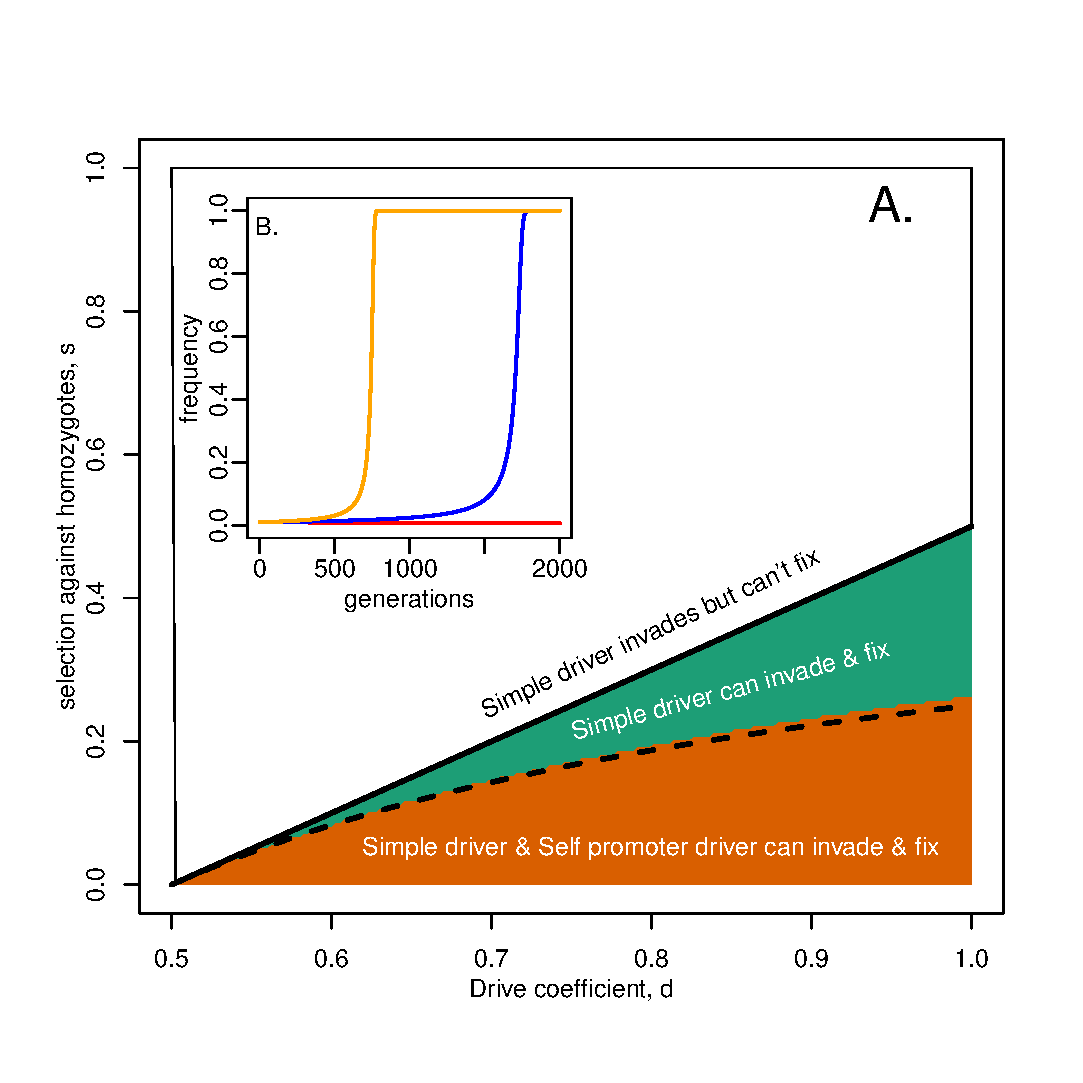
\includegraphics[width = 0.8 \textwidth]{Figures/invasion_space_recessive_driver.eps}
\caption{Invasion analysis. Likely merge with Figure 1. \yb{PERHAPS COMPARE TO TRADITIONAL DRIVER IN THIS FIGURE} } \label{Invasion_space}
\end{figure}


\subsection*{ sperm-egg haplotype balanced drive systems}

\begin{figure}
	\rotatebox{270}{\includegraphics[width = 0.8
          \textwidth]{Figures/sperm_egg_cartoon2.ps}}
\caption{transmission probabilities righthand allele through female
  meiosis}  \label{Eggsperm_3_allele_cartoon}
\end{figure}


\begin{figure}
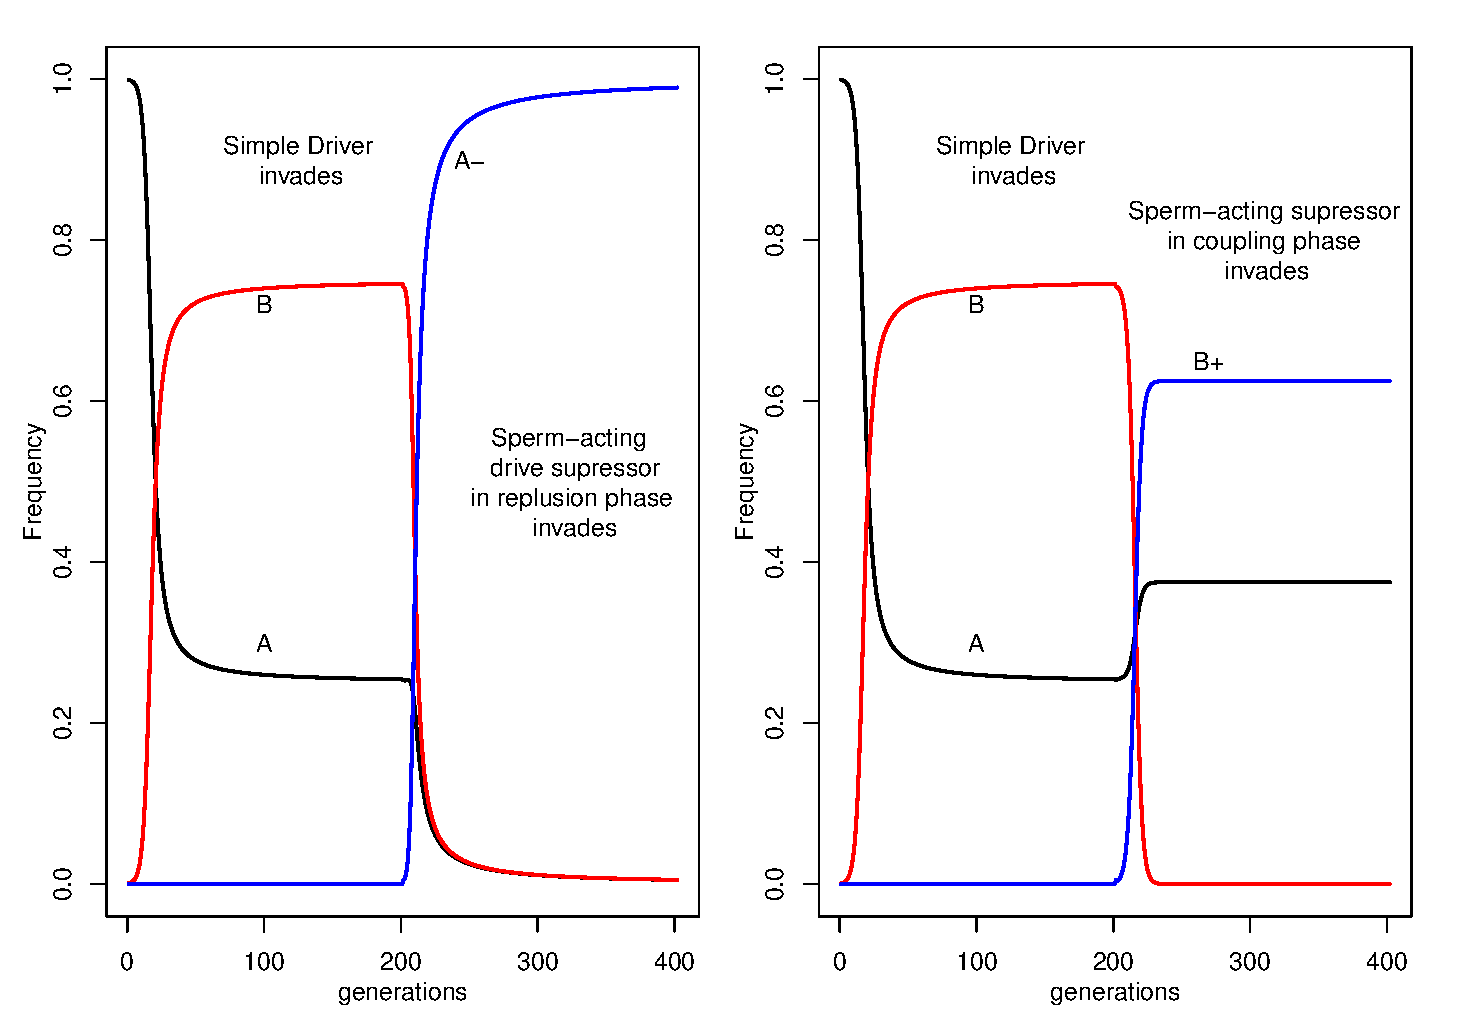
\includegraphics[width = 0.8 \textwidth]{Figures/trajectories_of_sperm_based_supressors.eps} 
\caption{Trajectories of two sperm-based supressors of drive. Possibly
merge this figure the 3 allele cartoon}  \label{Trajectories_of_supressors}
\end{figure}

Above, we explored a model were a driver that drove in females when signaled by a complementary allele in sperm.  
This complicated pleiotropic effect, while plausible is somewhat unlikely. 
Here, we examine an alternative scenario (and more realistic) in which
initially a driver, with no sperm-depedency, is at drive-viability equilibrium (with two alleles
$A$ and $B$ are the ancestral non-driver and driver alleles).
Subsequently a sperm-acting modifier of female meotic drive arises tightly
        linked to this balanced locus (effectively creating a third
        allele/haplotype at this locus).
Assuming tight linkage between female driver and sperm modifier is consistent with the nature of well characterized meiotic drive systems 
	which are often maintained as polymorphic inversions with numerous linked modifiers (CITE).


\yb{??In the SUPP we explore the dynamics of a sperm modifier of female drive unlinked to the female driver??} 


We will first consider the case where a sperm-acting facilitator of
female meiotic drive arises very tightly linked to the $B$ background 
creating the third allele $B^{+}$ (i.e. the non-recombining haplotype of a
        driver allele and sperm-acting drive modifier). 
This new allele which acts in sperm to increase the effectiveness of both
the $B$ and  $B^{+}$ drive in $AB$ and $AB^{+}$ heterozygotes, see Figure \ref{Eggsperm_3_allele_cartoon} for a simple schematic of this drive model.  
Naively this $B^{+}$ allele might be able to increase in frequency in the
population as then it could be allowed to spread due to the additional
drive it causes.
That turns out to not be the case, 
because the sperm-acting drive promoter (the novel $B^{+}$ haplotype) 
is introduced when the ancestral driver ($B$) is at drive-selection balance, 
	$B'$ will immediately suffer a homozygous fitness cost.  
Worse yet, a novel $B^{+}$ haplotype most often helps 
the $B$  allele drive ($B'$ sperm meeting $AB$ eggs), simply because $B$ is initially more common than $B^{+}$.
As $B^{+}$ facilitates $B$ these interactions will frequently form 
	$BB^{+}$ heterozygote that suffers from the full
	effect fitness costs as $BB$. 

Sperm-acting self promoting alleles are therefore at a profound disadvantage
in this scenario, even more so than under the previous two allele model.
We have found no parameter range of this
three allele system that allows the selfish sperm-acting allele $B^{+}$ to
invade the population. \yb{MATHS?}

While  sperm enhancement of a female drive cannot displace a polymorphic female driver, sperm based drive suppression - that is sperm-acting alleles that act to restore 
fairness of female meiosis can. 
 If these sperm-acting drive suppressors arise on
	the $A$ background (creating a third allele $A^{-}$) 
or are unlinked to the drive locus they readily invade a population segregating
for the drive system ($AB$, see Figure). The invasion of such allele
will lower the frequency of the original drive system (perhaps to zero)
and will spread to fixation if they do not carry strong fitness costs
(Figure \ref{Eggsperm_3_allele_cartoon} and \ref{Trajectories_of_supressors}A). \\


Intriguingly these sperm disruptors of female meiotic drive can spread
	even when they arise tightly linked to the original drive system (B), forming
	an novel third allele $B^{-}$ as above (Figures \ref{Eggsperm_3_allele_cartoon} and \ref{Trajectories_of_supressors}B). 
$B^{-}$ displaces the original drive system ($B$) because it drives when not costly, 
	but by disrupting drive when transmitted to sperm it avoids low-fitness drive homozygotes ($BB^-$ and $B^-B^-$. 
Surprising despite displacing the ancestral driver ($B$), self avoiding driver, $B^*$ it's equilibrium frequency is not always higher than that of $B$. 

\gc{Do we mention the In and Om locus here or in the discussion as a
	 potential e.g. Do we mention the fact that the frequency of these
	 newly invade sperm dodging alleles can be lower than the original system?}\\

\section*{Discussion}


Finally given a system of a balanced meiotic drive system which avoid
its own ill effects through a sperm-based mechanism
, such as that depicted in Figure XX and XX, female-based modifiers 
can evolve that act to further facilitate the sperms action in
disrupting driver. 

This logic may not hold for sex chromosomes. In ZW systems 
 Male modification of recombination rates
POssibility that this could happen in plants if pollen emit signals to ``egg''
Discussion of OM and IN.

Discussion of general conclusion that females have little reason to evolve supression mechanisms to prevent sperm influence on meiosis. 
General logic that sperm genome has to live in a zygote with consequences of its effect on female meiosis, so
it can not generate too dire a consequence.
I THINK THERE IS A MORE SUBTLE POINT . The sperm has special knowledge
that if it allows drive it will end up in the low fitness homozygote. 

\bibliography{refs}

\section*{Supplementary Stuff}

\begin{figure}
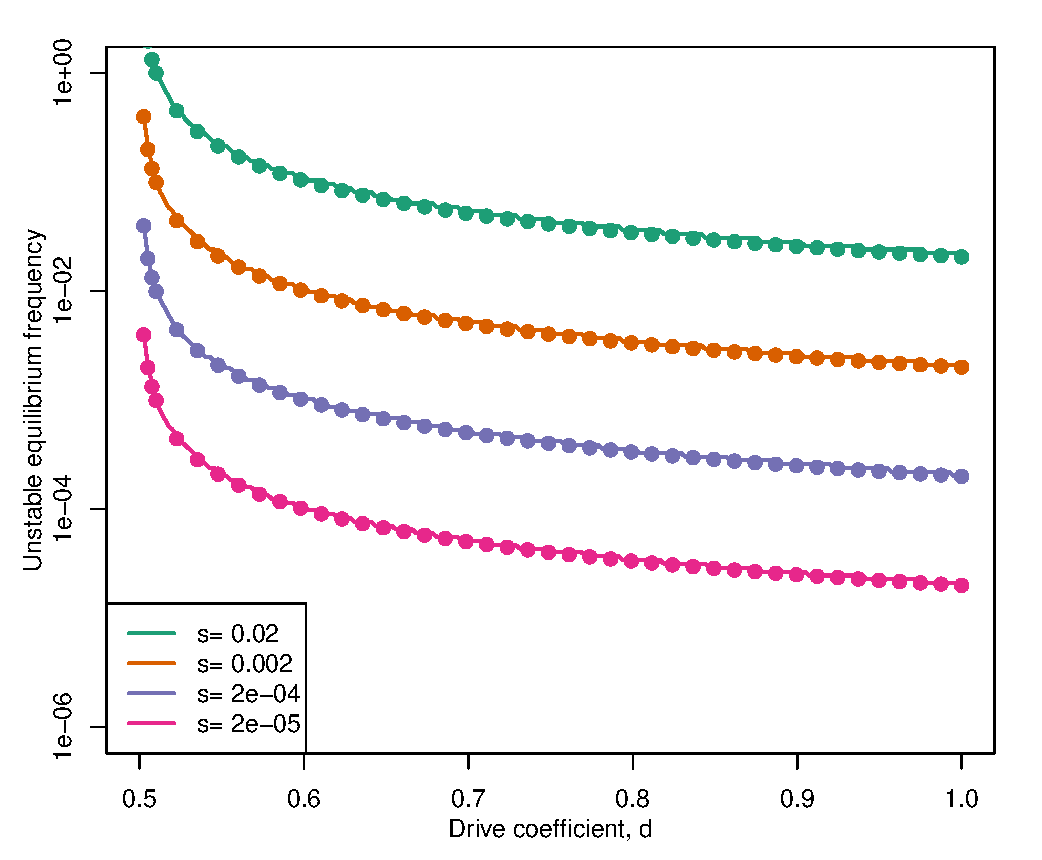
\includegraphics[width = 0.8 \textwidth]{Figures/bistable_x_vs_d_additive_s.eps} 
\caption{Bistable green-bearded allele when selection cost (s) acts
  additively, for an allele whose effect
 on female meoisis is mediated by sperm allele. }  \label{bistable_additive}
\end{figure}

\begin{figure}
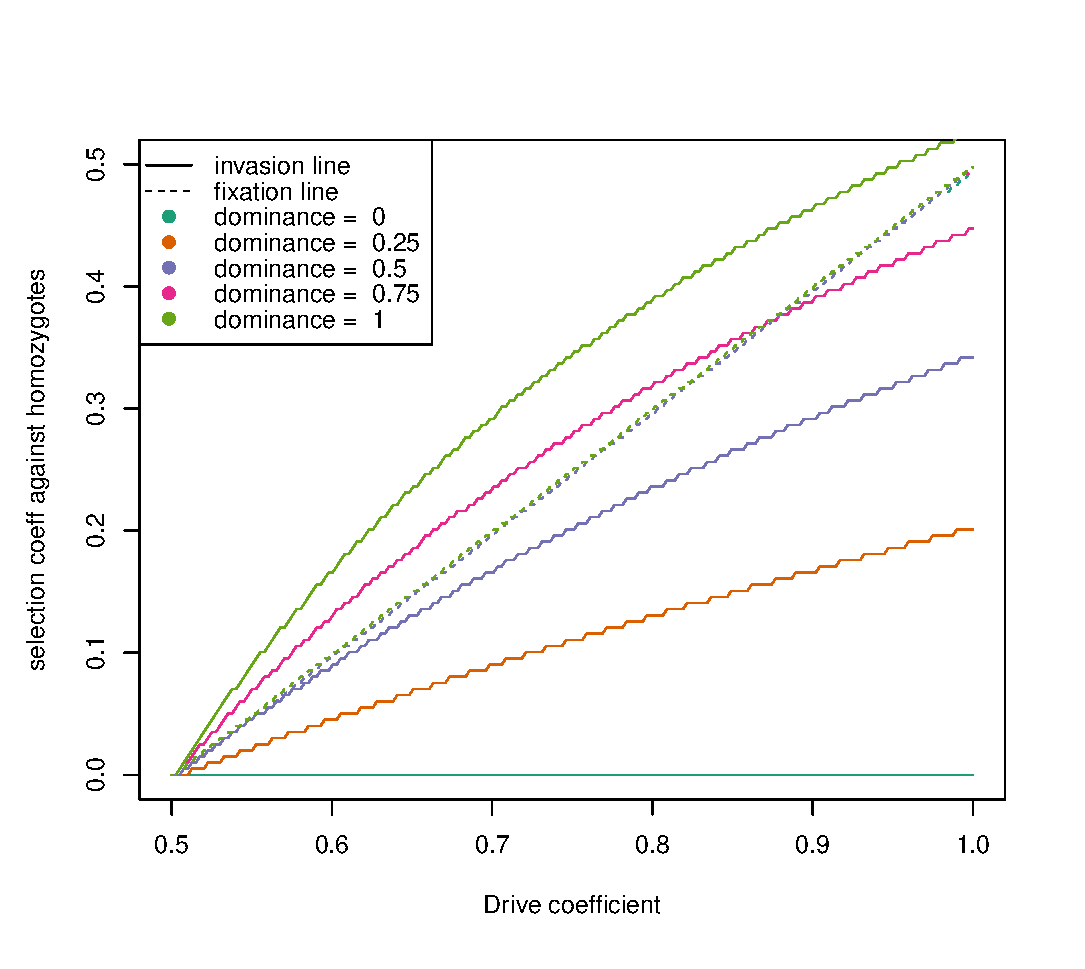
\includegraphics[width = 0.8 \textwidth]{Figures/effect_of_dominance_on_invasion_space_one_graph.eps} 
\caption{Invasion analysis of green-bearded sperm allele whose effect
 on female meoisis is mediated by the genotype of the fertilizing
 male. The area below the solid/dotted line is the parameter region
 where the allele can invade/fix (from $1/1000$ and $999/1000$
 \gc{maybe should lower this}). Note
 that all of the fixation lines are on top of each other as dominance
 parameter makes little difference here. The allele will be
 polymorphic in the parameter space where the solid (invasion) line
 falls above the dotted (fixation) line. Note that this is a very
 narrow parameter range, and only exists if the allele has a
 reasonable degree on dominance}  \label{Effect_of_dominance}
\end{figure}

\end{document}




\section*{OUTLINE}
\yb{YB: To me its (1) male enhancement of female drive cannot maintain a stable polymorphisms, and (2) An allele in sperm can evolve to suppress its drive in females.}
show that such alleles:
\begin{enumerate}
\item can't be balanced, \\
\item and homozygous problems are tested out at low freq.  \\
\item Any heterozygous problems, leads to a bistable allele\\
\item If these alleles take off they speed through to fixation\\
\item If allele has any drive ability in absence of sperm effect that is what allows it to enter the population
and sperm effect isn't a further cause of conflict. What if anything do we mean by this?\\
\item PERHAPS HERE WE INTRODUCE A SELF-RESTRAINING ALLELE
\end{enumerate}

Conclusion, such alleles are unlikely to cause evolution of female supressors, they test hemselves in a homozygous
state when they enter the population, and sweep quickly (all the way to fixation) if they enter the pop at all.\\


\begin{enumerate}
\item Setup a drive-selection balanced polymorphism in std. drive model. 
Do this by imagining the sperm-influence allele arising on the background of the driver, 
so the allele has drive capabilities, and can have had time to evolve new biology. 

Multilocus drivers held together with inversions, may offer a relatively large mutational/functional target.

Evolving on the new background means that the allele suffers the fitness consequences of the 
driver.  See A in Figure \ref{Eggsperm_3_allele_cartoon} \\
\item Sperm-based enhancers of drive can't invade (can they in some situations?). \\
\item Intuition is that the driver has already driven to a frequency 
where it is held in check by its cost in homozygotes. The sperm allele 
thus can't really help as it creates zygotes which suffer the homozygous fitness consequences.
\end{enumerate}

\subsection{So what can evolve?}
So what can happen?
\begin{enumerate}
\item Alleles that arise in linkage with drive systems, which when in sperm switch off drive, 
can spread. They benefit from drive, but avoid some of the
consequences ( (Bi) in Figure \ref{Eggsperm_3_allele_cartoon} ). Overall as a side product they are benefiting all in pop.\\
\item Presumably alleles that actually switch the allele that drives may do even better? As they'd end up in 
hets. Although they'd not drive, so hard to say. YB: There is evidence that In distorts meiosis in the other direction (they still drive when rare i.e. when not fused with drive supp sperm) \\
\item Alleles that cause sperm to switch off drive that arise on other background or unlinked to the drive system
are selected, and spread as fast as female supressors of drive ( (Bii) in Figure \ref{Eggsperm_3_allele_cartoon} )..\\
\item Alleles that in females facilitate the action of sperm supressors of drive (or vis versa) can spread. Haven't actually checked this.\\
\end{enumerate}

\section*{Conclusions.}